\documentclass{article}
\usepackage{mystyle}
\usepackage{amsmath, amssymb, amsfonts, amsthm, mathtools}
\usepackage[utf8]{inputenc}
\usepackage[inline]{enumitem}
\usepackage{cancel}
\usepackage{soul}
\usepackage{hyperref}
\usepackage{tikz-cd}
\usepackage{tikz}
\usetikzlibrary{decorations.markings, snakes}
\usepackage{changepage}
\usepackage{subcaption}
\usepackage[section]{placeins}
\usepackage{amsmath}
\usepackage{float}
\usepackage{gensymb}
\usepackage{graphicx}
\usepackage{adjustbox}
\graphicspath{./spaceflight mechanics images/}
\restylefloat{figure}


\theoremstyle{definition}
\newtheorem{theorem}{Theorem}[section]
\newtheorem{lem}[theorem]{Lemma}
\newtheorem{cor}[theorem]{Corollary}
\newtheorem{defn}[theorem]{Definition}


\setlength\parindent{0pt}
\let\emptyset\varnothing

\newcommand{\Int}{\operatorname{Int}}

\title{Spaceflight Mechanics}
\author{
  Hiya Akhil Gada\\
  19D100007\\
  Topic: Spaceflight Mechanics\\
  Mentor: Abhishek Raghuvanshi\\
}
\date{\today}
\smallauthor{Hiya Akhil Gada}

\begin{document}
\maketitle
\tableofcontents

\section{Particle Dynamics}

We shall revise a few basic laws of physics and derive a few formulae that will help us to fully understand the dynamics of spaceflight.

\subsection{Newton's Laws}

\begin{enumerate}
    \item A particle at rest remains at rest, and a particle in motion remains in motion, if the applied force is zero.
    \item The force on a particle equals mass times its inertial acceleration.
    \[\boldsymbol{F}= \frac{d\boldsymbol{p}}{dt} = m\boldsymbol{a}\]
    \item Every reaction has an equal and opposite reaction. 
\end{enumerate}





\subsection{Non-Inertial Frame of Reference}

Before we can go further, we must understand the mathematics that lies behind non-inertial frame of references, as spaceflight mechanics revolves around it. The calculations of the space vehicle are done on the reference frame of the earth, which is rotating and hence is non-inertial.

\subsubsection{Conversion}
We must know how to convert non-inertial frame co-ordinates to inertial frame coordinates. For that we use rotation matrices.


\begin{equation}\label{rot_mat}
 \begin{bmatrix} 
 A_{i1}\\
 A_{i2}\\
 A_{i3}\\
 \end{bmatrix} 
 =
 \begin{bmatrix}
 i_1\cdot s_1 & i_1\cdot s_2 & i_1\cdot s_3\\
 i_2\cdot s_1 & i_2\cdot s_2 & i_2\cdot s_3\\
 i_3\cdot s_1 & i_3\cdot s_2 & i_3\cdot s_3\\
 \end{bmatrix}
 \begin{bmatrix}
 A_{s1}\\
 A_{s2}\\
 A_{s3}\\
 \end{bmatrix}
\end{equation}

Where i is the inertial frame and s is the rotating frame.

\subsubsection{Velocity}
The relationship between the velocity with respect to the two frames is as follows:

\begin{equation}\label{vel_frame}
 \frac{^{i}d}{dt}\boldsymbol{r}=\frac{^{s}d}{dt}\boldsymbol r + \boldsymbol{w^{si}\times r}
\end{equation}

Where $\boldsymbol w^{si}$ the angular velocity of the s frame with respect to the i frame.

\subsubsection{Acceleration}

\begin{equation}\label{acc}
\begin{split}
  \frac{^{i}d^2}{dt^2}(\boldsymbol{R}+\boldsymbol{r}) & = \frac{^{i}d^2}{dt^2}\boldsymbol{R} + \frac{^{i}d}{dt}\left(\frac{^{s}d}{dt}\boldsymbol{r} + \boldsymbol{w^{si}\times r}\right)\\
  & = \frac{^{i}d^2}{dt^2}\boldsymbol{R} + \frac{^{s}d^2}{dt^2}\boldsymbol{r} + 
  2\boldsymbol w^{si}\times \frac{^{s}d}{dt}\boldsymbol{r} + \left(\frac{^{s}d}{dt}\boldsymbol{w^{si}}\right)\times \boldsymbol{r} + \boldsymbol w^{si} \times ( \boldsymbol w^{si} \times \boldsymbol{r})
\end{split}
\end{equation}

Using the equation \ref{vel_frame} we derive the above equation \ref{acc}.

The first term is the acceleration of the origin of s frame with respect to i frame, the second term is acceleration with respect to the s frame, the third term is called \emph{Coriolis force}, and the last term denotes the centripetal force.

\subsection{The Local Horizon Frame}
\begin{figure}[h]
    \centering
    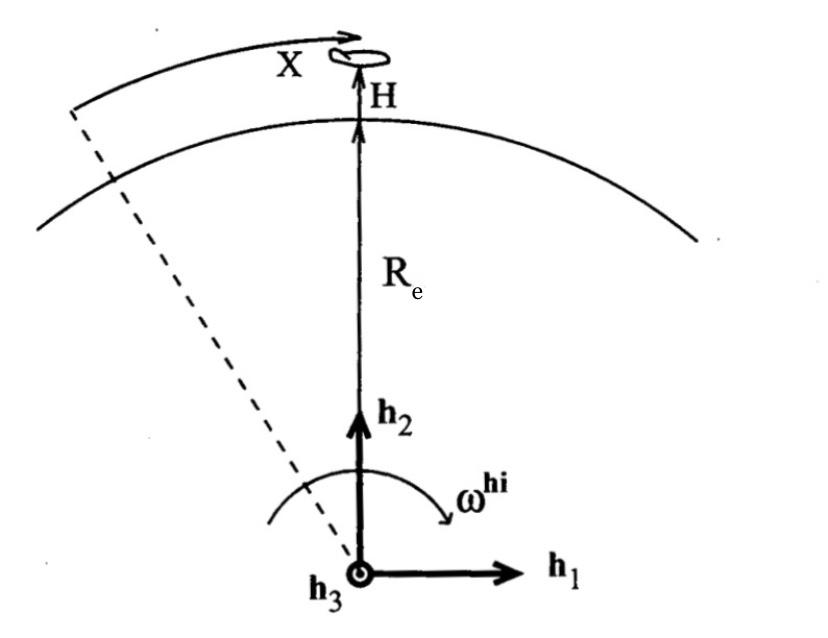
\includegraphics[scale=0.2]{image 1.jpeg}
    \caption{Local Horizon Frame}
    \label{fig:LHF}
\end{figure}


Let us consider the frame of reference, $\boldsymbol h$, given in the figure \ref{fig:LHF}. The inertial frame of reference is $\boldsymbol i$, at the centre of the earth. The rotation of the earth does not affect the unit vectors $\boldsymbol{h_1, h_2}$ and $\boldsymbol{h_3}$ significantly and is thus ignored. The $\boldsymbol h$ frame is such that the vehicle remains along $\boldsymbol{h_2}$ direction.

The position vector can be written as

\begin{equation}\label{pos_vec}
    \boldsymbol{r} = (R_e + H)\boldsymbol{h_2}
\end{equation}
\begin{equation}\label{omega}
    \boldsymbol{w_{hi}}= -\frac{\Dot{X}}{R_e + H}\boldsymbol{h_3}
\end{equation}

The inertial acceleration of the vehicle is as governed by equation \ref{acc_2}. 

\begin{equation}\label{acc_2}
    \frac{^{i}d^2}{dt^2}\boldsymbol{r}= \frac{^{h}d^2}{dt^2}\boldsymbol{r} + 
  2\boldsymbol w^{hi}\times \frac{^{h}d}{dt}\boldsymbol{r} + \left(\frac{^{h}d}{dt}\boldsymbol{w^{hi}}\right)\times \boldsymbol{r} + \boldsymbol w^{hi} \times ( \boldsymbol w^{hi} \times \boldsymbol{r})
\end{equation}

Each term in equation \ref{acc_2} is given by the following equations. The step-wise derivation is quite simple and has thus been skipped here.

\begin{equation}
    \frac{^{h}d^2}{dt^2}\boldsymbol{r} = \Ddot{H}\boldsymbol{h_2}
\end{equation}
\begin{equation}\label{dd0}
    \frac{^{h}d}{dt}\boldsymbol{w^{hi}}\times \boldsymbol{r}= \left(\Ddot{X} - \frac{\Dot{X}\Dot{H}}{R_e + H}\right)\boldsymbol{h_1}
\end{equation}
\begin{equation}\label{dd}
    2\boldsymbol w^{hi}\times \frac{^{h}d}{dt}\boldsymbol{r}= 2\frac{\Dot{X}\Dot{H}}{R_e + H}\boldsymbol{h_1}
\end{equation}
\begin{equation}
    \boldsymbol w^{hi} \times ( \boldsymbol w^{hi} \times \boldsymbol{r})= -\frac{\Ddot{X}^2}{R_e + H}\boldsymbol{h_2}
\end{equation}

The term in equation \ref{dd} is usually very small during launch and reentry and is ignored. If $\Dot{X}$ if large, then vertical speed $\Dot{H}$ is small and vice versa during launch and reentry. The same term in equation \ref{dd0} is also ignored. Thus we get the following equation.

\begin{equation}\label{main}
    m\left(\Ddot{X}\boldsymbol{h_1} + \left(\Ddot{H} - \frac{\Ddot{X}^2}{R_e + H}\right)\boldsymbol{h_2} \right) = -mg\boldsymbol{h_2} + \boldsymbol{L} + \boldsymbol{D} + \boldsymbol{T}
\end{equation}

Where $\boldsymbol{L}$ is the lift, $\boldsymbol{D}$ is the drag and $\boldsymbol{T}$ is the thrust. We will use equation \ref{main} often in the coming sections. 

Many other tools like conservation of energy and angular momentum are also used frequently instead of equation \ref{main}.

\section{Orbital Motion}

In order to predict the motion of spacecraft after the end point of ascent, we need to create a mathematical model that represents the motion of space craft.

To understand the orbital mechanics, we will revise the Kepler's laws and study them in detail. 

\subsection{Kepler's Laws}
\begin{enumerate}
    \item The planets orbit the sun in elliptical orbits, with the sun at one focus of the ellipse.
    \item The radius vector sweeps out equal area in equal times.
    \item The period of the orbit squared is proportional to the semi-major axis cubed.
\end{enumerate}

\subsection{Two body problem}
\begin{figure}[h]
    \centering
    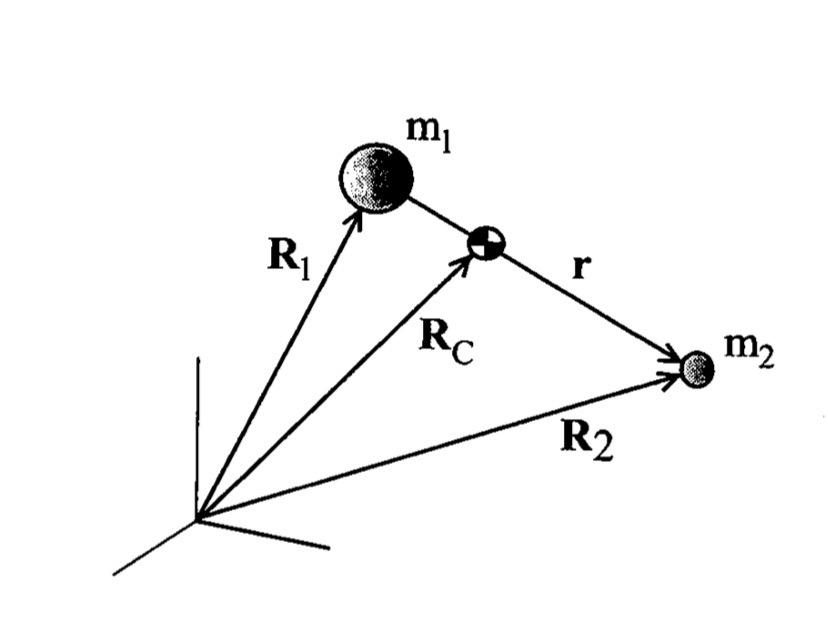
\includegraphics[scale=0.2]{image 2.jpeg}
    \caption{Two Body System}
    \label{fig:TB}
\end{figure}

The figure \ref{fig:TB} represents an inertial frame. To solve for the position vectors $\boldsymbol{R_1}$ and $\boldsymbol{R_2}$ we will need to solve six second order differential equations for each of the three components of $\boldsymbol{R_1}$ and $\boldsymbol{R_2}$.
Thus we need 12 constants, in total, to obtain the final solution. 

Instead of directly solving the equations we will take a different approach as follows. 

The net force on the system is zero. This means the acceleration of its centre of mass is 0. Thus,

\begin{equation}
\begin{split}
    m_1\boldsymbol{\Ddot{R_1}} + m_2\boldsymbol{\Ddot{R_2}} = 0 \\
    \Ddot{\boldsymbol{R_c}}=0
\end{split}
\end{equation}
This may be integrated twice to obtain
\begin{equation}
    \boldsymbol{R_c}= \boldsymbol{R_{c0}} + \boldsymbol{V_{c0}}t
\end{equation}

We have obtained 6 of the 12 required constants (3 each for the components of $\boldsymbol{R_{c0}}$ and $\boldsymbol{V_{c0}}$). 
For the remaining half of the solution let us consider the relative frame of the two bodies (with respect to $m_1$). 

\begin{equation}\label{rel_r}
    \Ddot{\boldsymbol{r}}= -\frac{\mu}{r^3}\boldsymbol{r}
\end{equation}

Where $\boldsymbol{r}$ is

\[\boldsymbol{r}= \boldsymbol{R_2}-\boldsymbol{R_1}\]

and $\mu$ is the conventional symbol for reduced mass.

The equation \ref{rel_r} shows acceleration of the second body in the relative frame. It can be computed by solving $\Ddot{\boldsymbol{R_1}}$ and $\Ddot{\boldsymbol{R_2}}$ using Newton's Gravitation Law. For the sake of brevity, the derivation has been skipped here. \medskip


Energy and angular momentum are conserved even in the relative frame of reference.
This statement can be proven mathematically by taking the dot product and cross product of the equation \ref{rel_r} respectively. 

Intuitively, conservation of energy makes sense as energy of a system always remains the same in any frame of reference. Angular momentum of this two body system is conserved as the force only acts along $\boldsymbol{r}$, i.e., there is no torque on the system. 

\subsection{The Orbit Equation}
We shall derive the orbit equation in this subsection. 
Lets start by taking the cross product with angular momentum per unit mass on either side of equation \ref{rel_r}.

\begin{equation}
\begin{split}
    \Ddot{\boldsymbol{r}}\times \boldsymbol{H} & = -\frac{\mu}{r^3}\boldsymbol{r} \times \boldsymbol{H}\\
    & = -\frac{\mu}{r^3}(\boldsymbol{r\times(r\times \Dot{r})}\\
    & = -\frac{\mu}{r^3}(\boldsymbol{r(r\cdot \Dot{r}) - \Dot{r}(r\cdot r)}
\end{split}
\end{equation}

$\boldsymbol{r\cdot r}= r^2$ and $\boldsymbol{r\cdot \Dot{r}}= r\Dot{r}$ (the component of velocity along the radius vector is the change in the magnitude of the radius vector itself) . Thus the equation can be re-written as

\begin{equation}
\begin{split}
    \frac{d}{dt}(\boldsymbol{\Dot{r}\times H}) & = \frac{\mu}{r}\boldsymbol{\Dot{r}} - \frac{\mu \Dot{r}}{r^2}\boldsymbol{r}\\
    & = \frac{d}{dt}(\mu \frac{\boldsymbol{r}}{r})
\end{split}
\end{equation}

Integrating both sides with respect to time and setting an integration constant as follows

\begin{equation}\label{e}
   \boldsymbol{\Dot{r}\times H} = \mu \frac{\boldsymbol{r}}{r} + \mu\boldsymbol{e} 
\end{equation}


Where $\boldsymbol{e}$ is called the eccentricity vector. The constant has been chosen as given above for convenience purposes, and its significance will become clear after the complete derivation.

Let's take dot product with $\boldsymbol{r}$ on either side.

\begin{equation}
    \boldsymbol{r\cdot \Dot{r}\times H} = \boldsymbol{r}\cdot \mu \frac{\boldsymbol{r}}{r} + \mu\boldsymbol{r\cdot e}
\end{equation}

The scalar triple product on the left hand side simplifies to $H^2$. Let us introduce the angle $\nu$ between the vectors $\boldsymbol{r}$ and $\boldsymbol{e}$. It is termed \emph{true anomaly}. On re-arranging the equation we get

\begin{equation}\label{r_pol}
    r= \frac{H^2/\mu}{1 + e \cos\nu}
\end{equation}

This equation is the polar form of a conic section with the origin at one focus.
We have proved that every two body system must travel along a curve which is a conic section with the eccentricity $e$. This proves Kepler's first law. 
The direction of the eccentricity vector can be found by proving that $r$ is smallest when $\nu = 0$. This means that $\boldsymbol{e}$ points to the \emph{perigee} of the orbit.

\subsection{Kepler's Equations}

\begin{figure}[h]
    \centering
    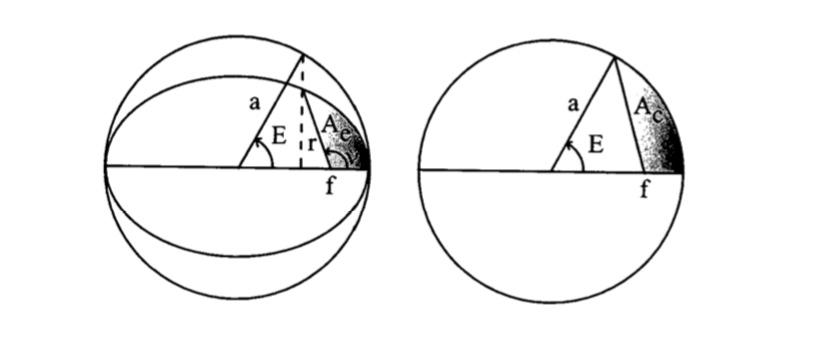
\includegraphics[scale=0.3]{image 3.jpeg}
    \caption{The eccentricity anomaly and auxiliary circle}
    \label{fig: aux_cir}
\end{figure}



Our ultimate aim now, is to find a solution of position with respect to time in a given orbit. Kepler introduced the auxiliary circle and the \emph{eccentricity anomaly E} as given in figure \ref{fig: aux_cir} for ease of calculation. 

We know that

\begin{equation}\label{A_e}
\begin{split}
    A_e & = \frac{b}{a}A_c\\
    & = \frac{ab}{2}(E-e\sin{E})\\
\end{split}
\end{equation}

We know that the rate of change of $A_e$ is constant. Thus equation \ref{A_e} can be related to time.

Consequently, Kepler's equation is given by 
\[M = E - e\sin{E}\]

Where M, called the mean anomaly, is defined as

\begin{equation}
\begin{split}
    M & = \sqrt{\frac{\mu}{a^3}}(t - T_0)\\
    & = n(t - T_0)
\end{split}
\end{equation}

(Here $T_0$ is the time of perigee passage). The Kepler's equation can be verified by solving the relation for $\frac{dA}{dt}$.

\subsection{The classical orbital elements}

To define an orbit, we must have $\boldsymbol{r}$ and $\boldsymbol{v}$. This means, to have six scalars in total. Classically, to define an orbit, we use a separate set of six scalars which shall be defined and discussed in this section.

\begin{figure}[h]
    \centering
    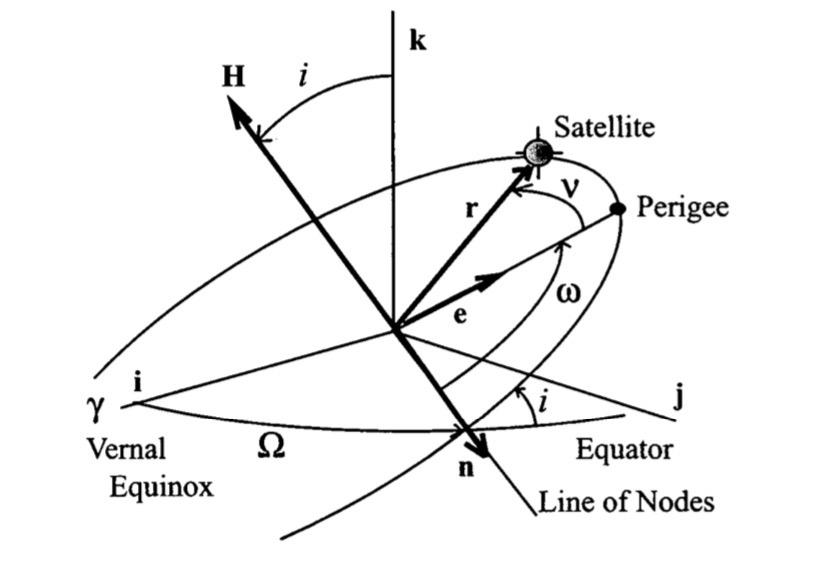
\includegraphics[scale=0.2]{image 4.jpeg}
    \caption{The classical orbital elements}
    \label{fig: classical terms}
\end{figure}


Referring to figure \ref{fig: classical terms}, these are:
\begin{enumerate}
    \item The semi-major axis $a$.
    \item The orbital eccentricity $e$.
    \item The time of perigee passage $T_0$.
    \item The right ascension of the ascending node $\Omega$.
    \item The orbital inclination $i$.
    \item The argument of the perigee $\omega$.
\end{enumerate}

First let us define the Line of nodes. It is the line which lies on the intersection of the orbital plane and the reference plane (here, the equatorial plane of the earth).

The $x$ axis always points towards the vernal equinox, the point on the sky where the sun crosses the equator from south to north on the first day of spring. The Greek letter $\gamma$ is used to denote this point.

The right ascension of the ascending node is the angle made by the ascending node from the $x$ axis.
The orbital inclination is the angle between the orbital plane and the reference plane.
The argument of the perigee is the angle between the  line joining the perigee to the  focus and the ascending node.
These six elements help to define the orbit and the motion completely. \medskip

We can easily calculate these terms by knowing the position and velocity at a given time (thus knowing the energy and angular momentum). 

This is shown briefly in the following equations.

\begin{equation}
    a = - \frac{\mu}{2\epsilon}
\end{equation}
Where $\epsilon$ denotes energy. The vector $\boldsymbol{e}$ can be found using equation \ref{e}.

\begin{equation}
    \boldsymbol{n}= \frac{\boldsymbol{k}\times \boldsymbol{H}}{|\boldsymbol{k}\times \boldsymbol{H}|}
\end{equation}
\begin{equation}
    \boldsymbol{n}= \cos{\Omega}\boldsymbol{i} + \sin{\Omega}\boldsymbol{j}
\end{equation}
\begin{equation}
    \cos{i} = \frac{\boldsymbol{k\cdot H}}{|\boldsymbol{H}|}
\end{equation}
\begin{equation}
    \cos{\omega} = \frac{\boldsymbol{n\cdot e}}{|\boldsymbol{e}|}
\end{equation}
\begin{equation}
    \cos{\nu} = \frac{\boldsymbol{e\cdot r}}{er}
\end{equation}

The explanation/derivation of these equations has been skipped for brevity.

What we have done till now is obtain six classical elements based on certain information at a given time.
To find the complete solution we must be able to find $\boldsymbol{r}$ and $\boldsymbol{v}$ at all points in time.
\medskip

We will only briefly talk about this method to get an intuitive feel without diving deep in the derivation.

We will first use Kepler's equation and use it to find $E$. We know the eccentricity and we know the $M$ (as we know the time).
Knowing $E$, we will use it to find $\nu$ (the true anomaly). The relation between $\nu$ and $E$ can be easily derived geometrically. 
This value is substituted in equation \ref{r_pol} to obtain $r$ at that time.
The vector $\boldsymbol{r}$ can also be found by the following relation.

\begin{equation}\label{orb_r}
    \boldsymbol{r}= r\cos{\nu}\boldsymbol{i} + r\sin{\nu}\boldsymbol{j}
\end{equation}

Where the origin is at focus.

And velocity is found by differentiating equation \ref{orb_r}. 
The relation $H = r(r\Dot{\nu})$ is used while solving for velocity. 

A number of approximation techniques are used to simplify the derivation like the \emph{Newton-Raphson method}.
Also sometimes $E=M$ is taken as an approximation, since the eccentricity of the orbit is very close to 0 (it is almost a circle).

\subsection{Earth Satellite Operations}

\subsubsection{The Hohmann Transfer}

The Hohmann transfer deals with the transfer of vehicles from one orbit to another.
This transfer is an optimal way to perform maneuvers. The only assumption taken is that the maneuver is impulsive.
This is a very good assumption as rockets are high thrust devices, and burn times are short compared to the time taken for vehicle movement.

\begin{figure}[h]
    \centering
    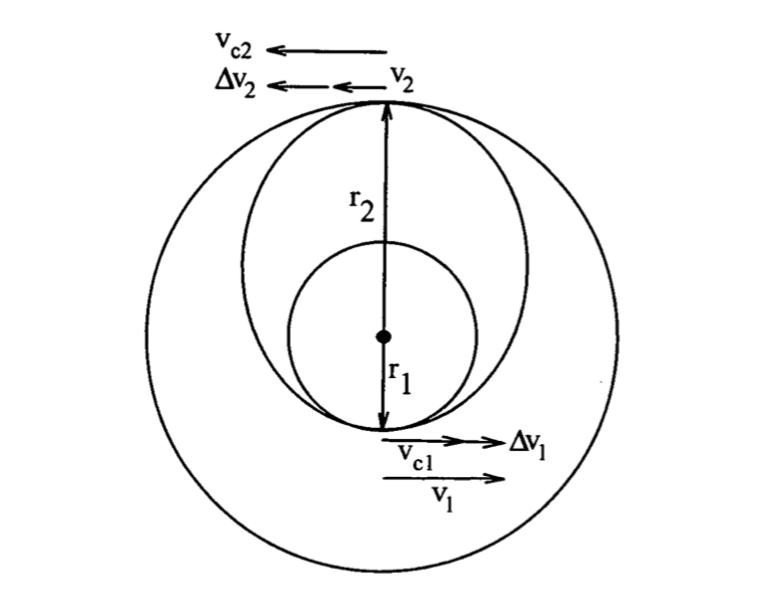
\includegraphics[scale=0.2]{image 5.jpeg}
    \caption{The Hohmann Transfer}
    \label{fig:HT}
\end{figure}


Refer to the figure \ref{fig:HT}. The objective is to transfer the vehicle from one circular orbit to another. 
Any orbit which passes through both the orbits can be used for transfer. 
If we use an orbit which goes further away from the earth than the outer orbit, it required extra energy, and hence is not that efficient. Conversely, if we use an orbit that descends lower than the inner orbit, energy is wasted to slow the vehicle down as it falls towards the earth.
\medskip

We also want to avoid spending energy in turning the velocity vector (although the initial and final energies may be same).
Thus intuitively, the most optimal orbit seems an elliptical orbit, tangent to both the circular orbits and which lies between the two circular orbits as given in the figure \ref{fig:HT}. 

Thus semi-major axis $a_t$ is thus
\[a_t = \frac{r_1 + r_2}{2}\]

There are two maneuvers involved, which changes the velocity of the vehicle at the points where the ellipse touches the two orbits. 
This needs to be done to impart sufficient energy for the vehicle to move in that particular orbit (first elliptical then circular orbit).

\subsubsection{Inclination Change Maneuvers}

A change in the orbit plane is one of the most expensive of all possible maneuvers. 
The maneuver must occur where the two planes intersect, i.e., the line of nodes.
The velocity change requirement is found by subtracting the two velocity vectors as shown in the figure \ref{fig:inc}

\begin{figure}[h]
    \centering
    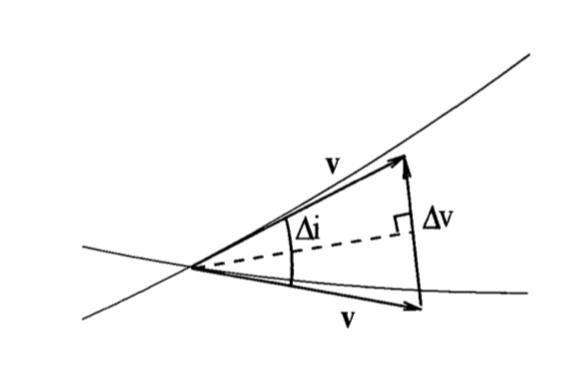
\includegraphics[scale = 0.3]{image 6.jpeg}
    \caption{Inclination change maneuver}
    \label{fig:inc}
\end{figure}

Thus 
\begin{equation}\label{vel_chng}
    \Delta v = 2v \sin{\frac{\Delta i}{2}}
\end{equation}

The velocity change given in equation \ref{vel_chng} can be very large. To give an idea, an inclination of $60\degree$ means $\Delta v = v$. This means the velocity change requires a booster, as powerful as the one that launched the payload in the first place.
It is thus vastly preferable to obtain the correct inclination during the original launch itself.
\medskip

Intuitively, satellite orbits with inclinations larger than the latitude of the launch site can be obtained by direct ascent trajectories. Thus the inclination change maneuver is used to obtain inclinations smaller than the latitude of the launch site.

If an inclination change is employed with a Hohmann transfer, then it is preferable to postpone the inclination change till the second maneuver as the velocity is lesser and thus the maneuver is less costly. 

\subsubsection{Launch to Rendezvous}

To launch a spacecraft to rendezvous another object already in orbit, like a space station, we have many options.
We can send the spacecraft in a particular orbit and then do an orbital inclination change maneuver. But this method is very expensive and is not preferred.
We can also do a "dogleg maneuver" which involves sending the vehicle some distance before sharply turning it into the required orbital plane. This method is also expensive as the velocity achieved before the sharp turn is largely wasted (energy is required to turn the velocity vector).
Notice that we only talk about bringing the vehicle into the particular orbit and not exactly at the point of the space station. This is because inter-orbit differences can be eliminated with phasing maneuvers\footnote{These are basically Hohmann transfers, which start and end at the same circular orbit, and whose time period is decided specifically so that the vehicle enters the original orbit at the right time.}. \medskip

The only efficient way to rendezvous with another orbiting space station is to launch when the space station \emph{orbit} passes directly overhead seen from the launch site as given in the figure \ref{fig:l_r}.

\begin{figure}[h]
    \centering
    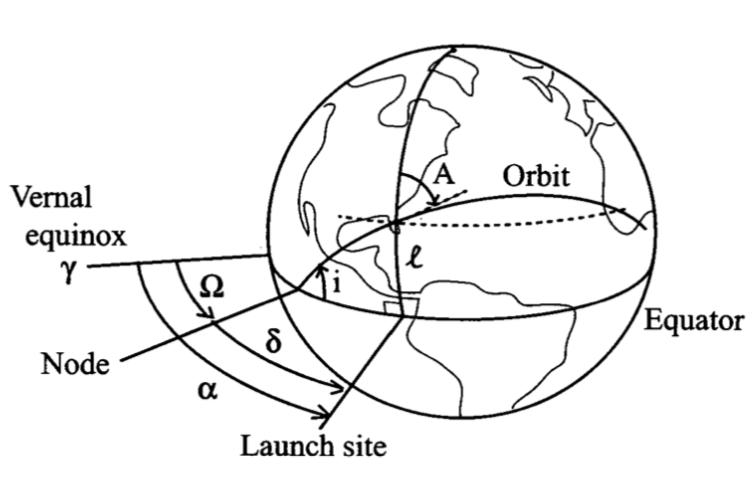
\includegraphics[scale=0.3]{image 7.jpeg}
    \caption{Launch to rendezvous}
    \label{fig:l_r}
\end{figure}

The dotted line in the figure \ref{fig:l_r} is called the \emph{ground trace} of the orbit plane projected on the earth's surface. We can clearly see that there will be two launch opportunities per day because of the earth's revolution.

The launch to rendezvous has to be done at the precise time (with an error of not more than a few seconds), leading to a very small "launch window".
It needs to be so precise that the precession of the orbit plane, must be also taken into consideration.

Another feasible, yet complicated method would be to launch the vehicle in a smaller orbit, and do a Hohmann transfer at the correct time to rendezvous with the space station in the outer orbit.

\subsubsection{Relative Motion and Rendezvous}

While performing maneuvers to rendezvous, to avoid the possibility of collision, some standoff distance is necessary.
So the vehicle is sent \emph{close} to the point of rendezvous and not exactly there.

The shuttle is now faced with the problem of closing the intervening distance to rendezvous. There exists a simple solution to this problem called the \emph{Clohessy-Wiltshire equations}. The derivation and the equations are skipped for brevity. 
The equation helps us model the motion of the shuttle to reach the space station.
The time for motion, can be varied over a reasonable range. So repeating the \emph{Clohessy-Wiltshire equations} for various time, and calculating the parameters for each case, we can find the one which leads to minimum energy rendezvous solution.

\subsection{Low Earth Satellite}
\subsubsection{Decay Lifetime}

Satellites in low earth orbits have finite lifetimes due to atmospheric drag.
Although the atmosphere may be almost perfect vacuum at that height, the satellite travels at high speed and the accumulated effects of drag over time get significant.

A satellite in orbit suffers an acceleration due to drag given by

\begin{equation}
    a_d = \frac{C_dA}{2m}\rho v^2
\end{equation}

Where $C_d$ is the drag coefficient, $A$ is the presented area of the satellite, $m$ is the mass of the vehicle, $\rho$ is the density of the atmosphere at that height, and $v$ is the velocity of the vehicle.

To calculate the decay lifetime, let us first assume that the first effect of drag on a satellite would be to circularize the orbit (if it is non-circular).
It also makes sense intuitively, as at the perigee, velocity is the most (initially), and is also close to the earth, leading to more drag.
The velocity decreases as it passes the perigee and lowers the apogee height almost as much as the perigee.

Thus now we are to solve only for the case of a circular orbit.
The air density is given by the formula
\begin{equation}\label{air}
    \rho = \rho_0e^{-(r-R_e)/h}
\end{equation}

Here $h$ is the atmospheric scale height\footnote{It is defined as the vertical distance over which the density falls by $1/e$. It is not the actual height, and is only taken as the height to satisfy the assumed model.}.
The equation \ref{air} is only used as an approximation.

Since we know $\epsilon = -\frac{\mu}{2a}$. When we differentiate it on both side with time, we get power on one side which is given by $-va_d$.
Hence,

\begin{equation}
    \frac{\mu}{2a^2}\frac{da}{dt} = -va_d
\end{equation}
Putting the value of $a_d$, integrating both sides and taking the assumption $R_e + H = R_e$, we get
\begin{equation}\label{decay}
    H(t) = h\ln{\left(e^{H_0/h} - \frac{\sqrt{\mu R_e}C_dA\rho_0}{mh}(t-t_0)\right) }
\end{equation}

\begin{figure}[h]
    \centering
    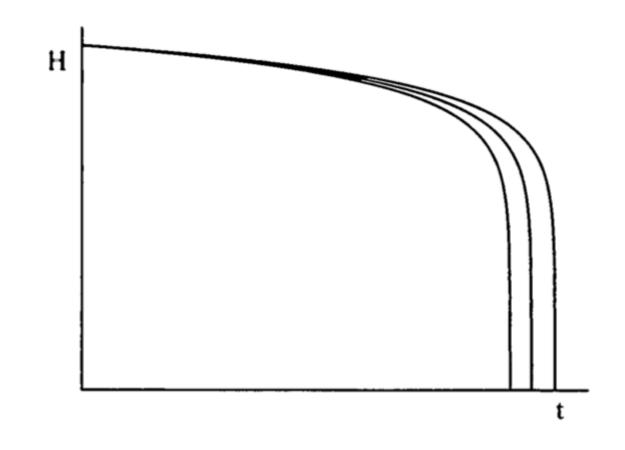
\includegraphics[scale = 0.2]{image 8.jpeg}
    \caption{Decay lifetime}
    \label{fig:decay}
\end{figure}

Note that $H$ and $h$ here are clearly different. In the integration $h$ is assumed to be constant. Using equation \ref{decay} we can find the decay lifetime.

In the analysis above, the assumption of the model for air density is the most questionable as air density is very erratic and changes with time and place. Even the practice of assuming $h$ as a constant throughout the trajectory is inaccurate.

However, the above analysis helps us to get a rough model. In practice, we seldom predict the decay time until about a week before decay and the final decay orbit cannot be predicted until a few hours in advance.

\subsubsection{Earth Oblateness Effects}

Because of Earth's rotation, it bulges at the equator by almost 20 km. This affects the orbit of a low earth satellite.
When the satellite is at points in its orbit furthest from the equator, the extra perturbing acceleration $a_p$ due to the bulge causes an average torque on the orbit. 
This torque is the same direction at both the most northerly and most southerly points in the orbit. Also when the satellite is crossing the equator, the extra mass simply increases the inward radial acceleration.

\begin{figure}[h]
    \centering
    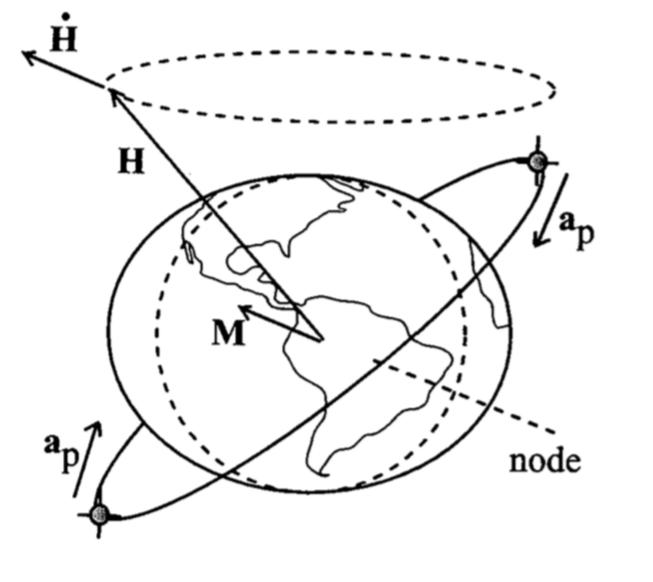
\includegraphics[scale=0.2]{image 9.jpeg}
    \caption{Earth oblateness effects}
    \label{fig:oblateness}
\end{figure}

Averaged over the entire orbit the torque $\boldsymbol{M}$ is not zero, and points towards the descending node.Refer figure \ref{fig:oblateness} This torque produces gyroscopic effects in the motion of the orbit, since it will make angular momentum "cone", just like in rotating top (according to $d\boldsymbol{H}/dt = \boldsymbol{M}$). This is sometimes also called $J_2$ perturbations or \emph{recession of the nodes} (as $\Omega$ is changing).

The second major effect is less obvious from the top analogy, but it occurs in the system as well. The elliptical orbit also rotates in its own plane.
This effect is also termed as the \emph{advance of the perigee} (as $\omega$ is changing).

To understand why and how such effects occur, i.e., $\Dot{\Omega}$ and $\Dot{\omega}$, we will have to see their mathematical derivation. You can refer to the notes of  Prof. H. Hablani under the course AE338 for the complete derivation.

\subsubsection{Other Perturbation Effects}

Sometimes for precision work, the Newtonian point mass potential $V= -\mu /r$ is replaced with the full geo-potential term

\begin{equation}
    V= -\frac{\mu}{r}\sum_{n=0}^{\infty} \sum_{m=0}^{n} \left(\frac{R_e}{r}\right)^n P_{n}^{m}(\sin{\delta}) (C_{nm}\cos{m\lambda} + S_{nm}\sin{m\lambda})
\end{equation}

Here $\lambda$ is the longitude and $\delta$ is the latitude; the $P_{n}^{m}$ are the associated Legendre polynomials. The earth's equatorial oblateness is from the $C_{20}$ term, which is related to $J_2$. Other terms also cause important effects in earth satellite motion.  
For example, the $C_{22}$, $S_{22}$ terms essentially model the earth's configuration of two major continental blocks. This term is the major driving force causing geosynchronous satellites to drift in longitude.

\subsection{Force Field in Space}

As space crafts operate mainly in our solar system, forces present in it need to be modelled suitably.
In this regard, it is useful to understand the nature of motion of planets, as these are also under similar forces.

In outer space, there is practically no atmosphere and therefore no aerodynamic forces are present.
Also, space craft has limited propulsion capability, which is used only for manoeuvres, resulting in no propulsive force.

Forces due to magnetic field and solar radiation are very small and have impact only on the long term drift of the satellite from its path.

Thus, gravity is the only important force, which primarily determines the space craft motion.
We use the universal law of gravitation.
In this gravitational model, we can invoke the \emph{spherical symmetry} and \emph{point mass} assumptions as size of planets are much smaller in relation to their mutual distances.

Sometimes a simplifying technique is used called the \emph{two-body simplification} wherein the gravitational pull of a body in the proximity is only considered. This reduces a complicated N-body problem to a two-body problem. 

The solution for this model has been already been discussed in previous sections.

Without loss of generality, we can assume larger body to be stationary, in cases where the centre of mass of the system is extremely close to the centre of the large body.

This results in what is commonly called a \emph{1-body problem} or \emph{central force motion}.

Here the origin becomes the centre of the larger planet.
The solution for this motion requires 6 initial conditions which are provided by the solution at the end of the ascent mission, in terms of position and velocity vectors of the space craft.


\subsection{Orbit Nature}

The orbit nature depends on the value of $e$ as discussed in previous sections.
It corresponds to the eccentricity of the orbit shape.

In cases where $e>1$, equation of conic corresponds to a hyperbola. In such cases the space craft escapes from the earth's gravitational field and attains inter-planetary path.

We have already discussed orbital solutions in terms of conic sections in previous sections.

\section{Launch Vehicles}

Now that we have briefly studied orbits and basic maneuvers, let us understand how the satellites are installed in the orbit using launch vehicles or rockets.
A space mission consists of 3 parts: ascent, orbital segment and re-entry.In this section, we will focus on ascent and how ascent is done using rockets.

\subsection{Ascent}

\subsubsection{Ascent Basics}

The object of ascent is to provide potential altitude, through a process that is safe and optimal.
Ascent not only involves design of the launch vehicle, but also of the trajectory
An ascent trajectory is broken into broad phases, based on nature of forces/ maneuvers.

\begin{figure}[h]
    \centering
    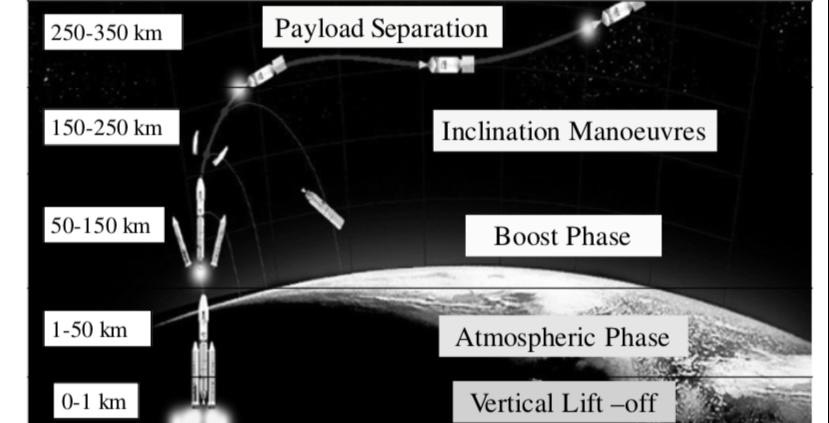
\includegraphics[scale=0.3]{sos picture.jpg}
    \caption{Ascent phases}
    \label{fig:asc}
\end{figure}

Refer to figure \ref{fig:asc}. We shall briefly discuss each stage. \textbf{Lift-off} is a critical phase, as toppling due to gravity is the major issue to tackle, while ensuring vertical attitude.
Once clear of the launch tower, boosters (or first stage engines) propel the vehicle through dense atmosphere (\textbf{Atmospheric phase}).
The \textbf{Boost phase} is solely to obtain large increments of velocity as the rocket is now out of atmosphere. Towards the end of this phase, maneuvers are carried out to rotate the velocity vector in order to achieve the desired terminal inclination (\textbf{Inclination maneuvers}).
The \textbf{Terminal phase/ Payload separation} is the most crucial as spacecraft separates after acquiring the required velocity and inclination.

\subsubsection{The Rocket Equation}

\begin{figure}[h]
    \centering
    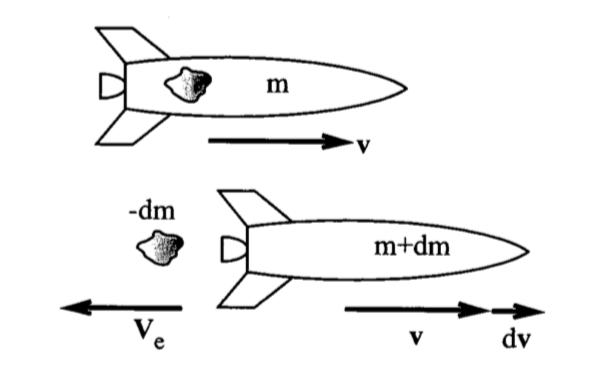
\includegraphics[scale=0.3]{image 10.jpeg}
    \caption{Conservation of momentum for a rocket}
    \label{fig:rocket}
\end{figure}

Consider the figure \ref{fig:rocket}. Assuming that there is no external force acting on the rocket, we can apply conservation of linear momentum.

\begin{equation} \label{lm}
\begin{split}
    (m + dm)(\boldsymbol{v} + d\boldsymbol{v}) - dm(\boldsymbol{v} + \boldsymbol{V_e}) & = m\boldsymbol{v} \\
    md\boldsymbol{v} - dm\boldsymbol{V_e} & = 0\\
\end{split}
\end{equation}

Here $\boldsymbol{V_e}$ is called the exhaust velocity of the rocket.
Dividing the equation \ref{lm} by $dt$ and realizing that there may be external forces, $\boldsymbol{F_{ext}}$ acting on the rocket, the equation \ref{lm} is modified to

\begin{equation}\label{lm2}
    \boldsymbol{F_{ext}} + \frac{dm}{dt}\boldsymbol{V_e} = m\boldsymbol{a}
\end{equation}

There is an additional term added to equation \ref{lm2}, when the rocket is operating in an atmosphere, or when the exhaust does not exist with zero pressure.

\begin{figure}[h]
    \centering
    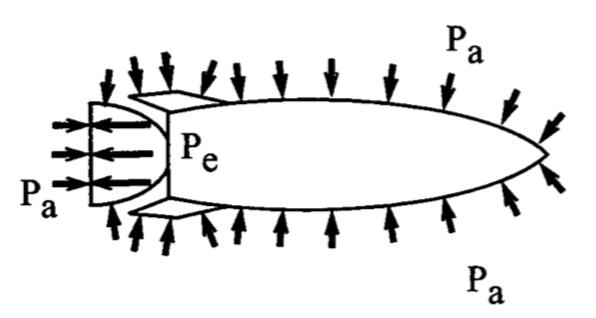
\includegraphics[scale=0.2]{image 11.jpeg}
    \caption{Atmospheric pressure effects on a rocket}
    \label{fig:atm press}
\end{figure}

As show in figure \ref{fig:atm press}, $P_a$ is ambient pressure, $P_e$ is exhaust pressure and the nozzle area is $A$.
Thus, the equation \ref{lm2} is modified to

\begin{equation}\label{lmfin}
    \boldsymbol{F_{ext}} + \frac{dm}{dt}\boldsymbol{V_e} - \frac{\boldsymbol{V_e}}{V_e}A(P_e - P_a) = m\boldsymbol{a}
\end{equation}

\subsubsection{Specific Impulse}

We define something called, specific impulse $I_{sp}$ which helps us compare the efficiency of different propulsion technologies. To a physicist, "specific" mean per unit mass, and the amount of momentum gained by the rocket per unit mass of fuel expended is 

\begin{equation}
    \frac{dm V_e}{dm} = V_e
\end{equation}

So, with this definition, specific impulse is really just exhaust velocity itself. However, according to engineering literature, specific impulse is the amount of momentum gained per unit \emph{weight} of fuel consumed.
Thus specific impulse is given as

\begin{equation}
    I_{sp} = \frac{dm V_e}{g_0 dm} = \frac{V_e}{g_0}
\end{equation}

Here $g_0$ is not the local acceleration of gravity, instead it is the standard acceleration of gravity on earth.

\subsubsection{Ideal Burnout Performance}

There are two tasks at hand. To design the vehicle, and to design the trajectory.
These both depend on each other and thus it is difficult to find an absolute relation between the two.
The method we follow is iterative: we first characterize the trajectory nature and get the first design model, then we proceed to design the vehicle and so on the iterations continue till a satisfactory result is obtained.
In the first steps, most models and solutions we arrive at use idealized scenarios to capture the primary effects. Subsequently, these primary solutions are corrected for the secondary and tertiary physical effects during iterations.

We will now define an ideal scenario called the \emph{Ideal Burnout Performance} and is obtained under force-free assumption.

From equation \ref{lmfin} the equation for this model would be

\begin{equation}\label{ib}
    \frac{d\boldsymbol{v}}{dt} = -\frac{\Dot{m}}{m} g_0 I_{sp} \boldsymbol{u_v}
\end{equation}

Where $\boldsymbol{u_v}$ is a unit vector in the direction of $\boldsymbol{v}$.

Ideal burnout velocity ($\boldsymbol{V_b}$) obtained after integrating equation \ref{ib}, is the maximum velocity that a rocket will generate from given propellant and structural mass.
Gravity and atmospheric drag typically reduce $\boldsymbol{V_b}$. 

\subsubsection{Gravity and Drag model}

We see there are two kinds of losses in the ascent of a vehicle. The loss due to drag and gravity, and the loss in the form of kinetic and potential energy of the burnt mass as well as the mass of the rocket minus the payload.

We will briefly discuss a gravity model and a drag model.

For gravity, the correct method to find height of the vehicle at a time $t$, would be to find velocity by integrating equation \ref{lmfin} (assuming zero pressure difference) and then by integrating the velocity with respect to time.

Thus we need to solve these two equations

\begin{equation} \label{grav model}
\begin{split}
    \frac{dv}{dt} & =  -\frac{\Dot{m}}{m} g_0 I_{sp} - g   \\
    h(t) & = \int v dt
\end{split}
\end{equation}

(Here $g$ is the local acceleration due to gravity which depends of $h(t)$).

The integration is difficult to solve as $g$ itself depends on height. For this we devise a simplified model.
We assume that $g$ is constant, and then solve the equations, to finally obtain height. 
Then, we find the "correct" $g$ value using the height, and then repeat the entire process again.
We perform these iterations till the change in the values of $g$ is small enough.

For drag, the complexity lies in the erratic atmospheric density and other factors, which make drag very difficult to graph.
For this we assume a constant average deceleration, based on total energy loss. This gives a reasonable performance estimate. Thus the equation \ref{grav model} becomes 

\begin{equation}
    \frac{dv}{dt} =  -\frac{\Dot{m}}{m} g_0 I_{sp} - g - \frac{D}{m}
\end{equation}

Here $D$ is the drag on the launch vehicle.

\begin{figure}[h]
    \centering
    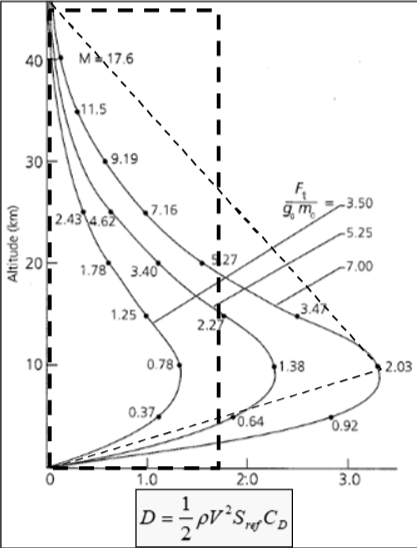
\includegraphics[scale=0.6]{image 13.png}
    \caption{Drag Model}
    \label{drag model}
\end{figure}

As you can see in the figure 13, the graph of altitude against drag is converted first into a triangular approximation, which is the converted into a rectangular plot (so as to obtain the average acceleration).


\subsubsection{Inclined/Curvilinear Trajectories}

In reality, vertical motion is used only for a very small part of the overall ascent mission. 
For the most part, ascent trajectory is inclined and curvilinear in nature.
This is mainly because one of the terminal constraint is that the inclination should be zero or close to it. \medskip

Consider a rocket as given in the figure \ref{fig:inclination}

\begin{figure}[h]
    \centering
    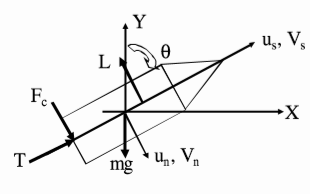
\includegraphics[scale=0.6]{image 12.png}
    \caption{Effect of Inclination}
    \label{fig:inclination}
\end{figure}

We need a force normal to the length of the rocket, for it to follow a curvilinear path. 
According to figure \ref{fig:inclination} this force is provided by a component of the weight of the rocket. All the other forces are along the length of the rocket.
In this case, (when $\boldsymbol{L} = 0$ and $\boldsymbol{F_c} = 0$) the resulting trajectory is called \emph{Gravity Turn} trajectory, as $g$ alone is responsible for turning.

The scalar equations of planar motion, in the absence of $\boldsymbol{L}$ and $\boldsymbol{F_c}$ are as follows 

\begin{equation}\label{motion1}
\begin{split}
    a_s & = \frac{dV}{dt}\\
    & = - \frac{\Dot{m}}{m} g_0 I_{sp} - g \cos{\theta}
\end{split}   
\end{equation}

\begin{equation}\label{motion2}
\begin{split}
   a_n & = V \frac{d\theta}{dt}\\
   & = g \sin{\theta}
\end{split}   
\end{equation}


Conceptually, we can solve for any 2 of the 3 quantities ($V, \Dot{m}, \theta$), provided the third one is given.

To obtain the trajectory and the vehicle design for such a problem is very complex. Therefore for early design stage, analytical solutions are found to be more useful for gross vehicle sizing. 
It helps us in quick assessment of various concepts, before selecting the best for detailed analysis. \medskip

Among the many possibilities of generating analytical solutions, there are three which are simple and elegant. 

As most launch vehicles use some kind of control during ascent, it is possible to specify a constant value for $\frac{d\theta}{dt}, \frac{\boldsymbol{T}}{m}$ or $V$. This will be the basis of our analytical solutions. 

\subsection{Ascent Solutions}

\subsubsection{Constant q solution}

The \emph{pitch rate} $q_0$ is defined as 
\[\Dot{\theta} = q_0\]

We obtain V(t), using the equation \ref{motion2}, as follows
\begin{equation}\label{q_vsoln}
\begin{split}
    \Dot{\theta} & = \frac{g \sin{\theta}}{V(t)}\\
    V(t) & = \frac{g \sin{\theta}}{q_0}
\end{split}
\end{equation}

This equation shows us that analytically, $V(t)$ is higher for higher $\theta$ and for lower $q_0$.

However, this equation has a few faults. In the equation \ref{q_vsoln}, $\theta$ can not be $0$. This simply means that gravity turn can only be started from a non-zero $\theta$ after it has acquired finite $V$.
This requirement is usually met by giving a \emph{pitch kick} to the vehicle.

We obtain the solution for $m(t)$ as follows
\begin{equation}
    \Dot{V} = \frac{d}{dt} \frac{g \sin{\theta}}{q_0} = g\cos{\theta}
\end{equation}
Now we put this in equation \ref{motion1} and obtain
\begin{equation}
\begin{split}
    \frac{dm}{m} & = - \frac{2 g \cos{\theta} d\theta}{q_0 g_0 I_{sp}}\\
    \ln{\frac{m_0}{m}} & = \frac{2 g \sin{\theta}}{q_0 g_0 I_{sp}}(\sin{\theta} - \sin{\theta_0})
\end{split}
\end{equation}

This indicates that for small $q_0$ large $m_0$ is needed to achieve terminal conditions. 
Also a large $q_0$ will reduce terminal velocity. 
Therefore the design of ascent mission under constant $q_0$ needs its careful selection.

\subsubsection{Constant V solution}

Gravity turn can also be employed, when the vehicle has reached a desired velocity but does not have inclination.

For $\theta(t)$ we use the equation \ref{motion2} to get

\begin{equation}\label{v_theta.const}
\begin{split}
    \frac{d\theta}{\sin{\theta}} & = \frac{g}{V_0} dt\\
    \tan{\frac{\theta}{2}} & = \tan{\frac{\theta_0}{2}} e^{\frac{g \Delta t}{V_0}}
\end{split}
\end{equation}

We see that higher $\Delta t$ would give higher $\theta$.

The mass solution for constant $V$, using equation \ref{motion1}, is

\begin{equation}
\begin{split}
    \Dot{V} & = 0 \\
    \frac{dm}{m} & = -\frac{g V_0}{g_0^2 I_{sp}} \frac{\tan{\theta}}{d\theta} \\
    \frac{m}{m_0} & = \left(\frac{\sin{\theta}}{\sin{\theta_0}}
\right)^{-\frac{g V_0}{g_0^2 I_{sp}}}\\
\end{split}
\end{equation}

Thus a higher $\theta$ results in higher propellant to be burnt.

\subsubsection{Constant T/m Solution}

While constant burn rate design is easy to implement, it results in increased forward acceleration, causing large compressive loads on the rocket.
A way to avoid such a situation is to reduce the thrust as mass reduces so that net forward acceleration remains within acceptable bounds.

Specific thrust, defined as $\boldsymbol{T}/m$, is the amount of acceleration that propulsion generates.

For the solution of $V$, we use both the equations \ref{motion1} and \ref{motion2}
\begin{equation}
\begin{split}
    \Dot{V} & = \frac{T}{m} - g\cos{\theta}\\
    V & = g\sin{\theta} \\
    \int{\frac{dV}{V}} & =  - \int{\tan{\theta} d\theta} + \frac{T}{m} \int{\frac{d\theta}{\sin{\theta}}}
\end{split}
\end{equation}

\begin{equation}
    \ln{V} = \ln{\cosec{\theta}} + \frac{T}{m} \ln{\tan{\frac{\theta}{2}}} + C
\end{equation}

For the solution of $m$, we use the definition of $I_{sp}$ 

\begin{equation}
\begin{split}
    \int{\frac{dm}{m}} & = - \frac{T g}{m g_0 I_{sp}} \int{dt}\\
    \ln{m} & = - \frac{T g}{m g_0 I_{sp}} t + C 
\end{split}
\end{equation}

If we intend the velocity to increase continuously, the net forward acceleration must be positive at all times. This is possible if $T/m$ is greater than $\cos{\theta}$ at all times (thus greater than 1 at all times).

Constant $T/m$ based solutions show that for larger value, it takes more time and propellant to achieve the same $\theta_b$ ($\theta$ at burnout).
However, it also results in larger terminal velocity. 

\medskip


 
\begin{tabular}{||c|c|c||}
    \hline
    Constant $q_0$ Solution & Constant $V$ Solution & Constant $T/m$ Solution \\
    \hline
    Small $q_0$, $m_0$ increases. & If $\theta_b$ is high, $\Delta t$ and propellant  & If $T/m$ is high, $\Delta t$ and propellant \\
     Large $q_0$, $V_{terminal}$ is lower. & mass consumed is more. & mass consumed is more \\
     & & (more than constant $V$ solution).\\
    \hline
    Compressive stresses  & Lower stresses & Controlled stresses\\
    \hline
    Simple to implement & Can be employed even  & Terminal velocity is high\\
    & when $\theta=0$, unlike  & \\
    & constant $q_0$ solution & \\
    \hline
\end{tabular} \medskip

\subsection{Multistage Rockets}

We combine the ideal burnout concept along with the gravity and drag loss models.
In general we can find out the specifications of the rocket like its initial mass using this method.

Till now we have assumed that all the propellant is burnt at one go. 
Such rockets are called single stage rockets and are employed to launch small-sized spacecraft, as payload fractions are small for such operations. \medskip

For a more efficient rocket configuration, we use the concept of multistage configuration.
Energy imparted to the shell as well as the unburnt propellant are a complete loss for the mission.
In this context, we must keep it in mind that single stage payloads are a fraction of 0.001, resulting in a very inefficient mission.
Multistage rockets aim to address this deficiency.

Multi-staging means dividing the total rocket into sub-rockets called \emph{stages}.
At the end of burnout of each stage, the shell is separated from the rest of the rocket.

Thus after each stage is over, starting mass for next stage is significantly smaller, causing a reduction in energy due to loss due to gravity (and other losses).

It allows us to use dissimilar technologies in the same vehicle mission (like propellant or structure).

Multistage rockets are very complicated to design. Staging issues occur if the number of stages is more than 4.
More the separation points on a rocket more the precision in engineering required and more the chances of a catastrophic event mid-flight.

\subsubsection{Multistage Design Concept}

Consider the following notation:

Lift-off Mass: $m_0 = \sum_{i=1}^n m_{pi} + \sum_{j=1}^n m_{sj} + m_*  $

Stage-wise starting mass: $m_{0i} = m_{pi} + m_{si} + m_{0i+1} $

Stage-wise ending mass: $m_{fi} = m_{si} + m_{0i+1} $

Stage-wise specific impulse: $I_{sp}$

\begin{figure}[H]
    \centering
    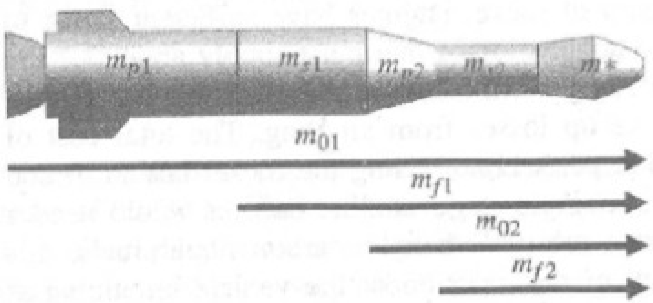
\includegraphics[scale=0.3]{image 14.png}
    \caption{ A multistage rocket }
    \label{fig:multistage}
\end{figure}

For the $i^{th}$ stage operation of an N-stage rocket, the sum of masses of  all the stages from ‘i+1’ to ‘N’ and the final payload mass, is treated as its payload.

Inert mass of $i_{th}$ stage is separated after its burnout but before the operation of the $i+1_{th}$ stage is begun. \medskip

Three staging parameters are defined as below:

Stage-wise payload ratio: $\pi_i = \frac{m_{0i}}{m_{0i+1}}$

Stage-wise structural ratio: $\epsilon_i = \frac{m_{si}}{m_{si}}  $ \medskip

While,$\epsilon_i$ denotes the status of structural technologies and $I_{spi}$ captures the status of propulsion technologies, $\pi_i$'s indicate how $m_0$ is distributed between stages.
 
\subsubsection{Multistage formulation}

In this context, generally $I_{spi}$ and $\epsilon_i$ are available as a set of discrete values, based on technological options.
Thus, the design solution involves only the $\pi_i$'s as unknowns.

Thus, formulation starts by defining mission payload ratio, $\pi_*$, in terms of stage payload ratios, $\pi_i$, as follows.

\begin{equation}
    \pi_*= \frac{m_*}{m_{0}} = \frac{m_*}{m_{0n}} \times \frac{m_{0n}}{m_{0(n-1)}} \times \ldots \times \frac{m_{02}}{m_{01}}  = \prod_{i=1}^n \pi_i
\end{equation}

Ideal burnout velocity for a multistage rocket is nothing but the sum of ideal velocities as shown below.

\begin{equation}
    V_0 = \sum_{i=1}^n \Delta V_i = -\sum_{i=1}^n g_0 I_{spi} \ln{\frac{m_{0i} - m_{pi}}{m_{0i}}}
\end{equation}

As masses can be expressed in terms of $\pi_i$'s and $\epsilon_i$'s, we can also obtain the velocity in terms of these.

The derivation has been skipped for brevity.

\begin{equation}
    V_0 = -\sum_{i=1}^n g_0 I_{spi} \ln{(\epsilon_i + \pi_i\times (1 - \epsilon_1))}
\end{equation}

As has been noted earlier, rocket mass configuration, including its stages,is a function of payload ratios,$\pi_i$'s.
Further,we have also seen that different values of these ratios result in different lift-off mass as well as stage wise masses,for same payload,propulsion and structure.

The design task is thus, to choose among the many combinations, the one which results in the best rocket. Optimal techniques aim to achieve this objective.

\subsubsection{Optimal design methodology}

In multi-stage rocket design, basic design variables are masses within each stage.
In most cases, objective is to maximize, either $m_*$ for a given $V_*$, or vice versa, thus obtaining the objective function. 
The other is taken as the constraint.
In all these cases, number of stages is used as a parameter.

Gradient based methods are used to optimize the objective function.
In gradient based methods, partial derivatives of objective function, with respect to design variables, are driven to zero,while satisfying the constraint exactly.
Thus, for an N stage vehicle having N design variables, we have N+1 equations, for N unknowns. \medskip

We use the Lagrange multiplier concept. 
We know that solution will be optimal only at a point where all derivatives are zero simultaneously.
Here we introduce the concept of constraint error that needs to be accounted for, while generating derivatives. 
This is achieved by augmenting the objective function through the addition of a term corresponding to the constraint error, through an additional unknown called the Lagrange multiplier which acts the weight for the error.
In this manner, partial derivatives of the augmented objective function include the effect of error due to inexact satisfaction of constraint. \medskip


Given below are the two basic equations of the two objective functions, for a rocket with N stages.

\begin{equation}
    \ln{\pi_*} = \sum_{i=1}^N \ln{\pi_i}
\end{equation}
\begin{equation}
    V_* = - g_0 \sum_{i=1}^N I_{sp} \ln{(\epsilon_i + (1 - \epsilon_i)\pi_i)}
\end{equation}

Constraint errors are as defined below. 
\begin{equation}
    e_\pi = \ln{\pi_*} - \sum_{i=1}^N \ln{\pi_i}
\end{equation}
\begin{equation}
    e_V = V_* + g_0 \sum_{i=1}^N I_{sp} \ln{(\epsilon_i + (1 - \epsilon_i)\pi_i)}
\end{equation}

Augmented objective functions are as defined below.
\begin{equation}
    \ln{\pi_*} = \sum_{i=1}^N \ln{\pi_i} + \lambda(V_* + g_0 \sum_{i=1}^N I_{sp} \ln{(\epsilon_i + (1 - \epsilon_i)\pi_i)}) = H_\pi(\lambda, \pi_i)
\end{equation}
\begin{equation}
    V_* = - g_0 \sum_{i=1}^N I_{sp} \ln{(\epsilon_i + (1 - \epsilon_i)\pi_i)} + \lambda(\ln{\pi_*} - \sum_{i=1}^N \ln{\pi_i}) = H_V(\lambda, \pi_i)
\end{equation}

It is clear that partial derivatives of the above functions contain both objective and constraint related information. \medskip

The procedure for solving the optimal rocket sizing problem is given below.

\begin{enumerate}
    \item All the N partial derivative equations are solved for $\pi_i$'s in terms of Lagrange multiplier $\lambda$.
    \item Next, the $\pi_i$'s are substituted into the constraint equation and value of $\lambda$ is obtained.
    \item We use this value to find the $\pi_i$'s.
\end{enumerate}

The final result of the \emph{Lagrange solution} has been skipped for brevity. \medskip

The Lagrange procedure has a limitation that the equation for $\lambda$ is an $N^{th}$ order algebraic equation, so that solution requires more effort for more number of stages.

Also when both $\epsilon_i$ and $\pi_i$ are distinct (unequal stages), the solution requires additional effect.

Therefore, it would be useful if we can set up a simpler process, which does not compromise significantly on the accuracy.

\subsubsection{Approximate staging concept}

It is possible to get good solutions if we drop one equation and then solve the resulting square system.
While, there can be many options for dropping one equation, this can be achieved exactly, if one of the partial derivatives is zero throughout the design space. 
We assume here that there is only one point in design space where the objective function is a maximum.
In such a case, the point automatically represents optimal design solution, at which all partial derivatives go to zero. \medskip

In this method, as constraint needs to be satisfied exactly, the corresponding equation is used to express one design variable in terms of all other remaining variables.
This solution is then substituted in the $N-1$ partial derivative equations.
The derivative corresponding to the selected design variable is ignored.
Once this system is solved, these are substituted back into the constraint and the $N^{th}$ variable is solved for.

\subsection{Concept of variants}

There are many situations where an optimally designed configuration needs to be modified for a marginally different mission. 
This could be either in terms of a slightly higher burnout velocity or more commonly, a higher payload.

In general, such requirements are addressed by slightly modifying optimal configuration to ensure that modified configuration also remains optimal.

Typically, a variant is created by modifying/ replacing an existing stage in terms of structure, propellant mass or its specific impulse.
The modifications/ replacements are usually a small fraction of the existing stage, in order to minimize impact on other design/ operational aspects.

\subsubsection{Trade-off ratio concept}

Trade-off ratios indicate how a small change in the stage configuration affects performance, and thus, establish the robustness of the design.
They also provide a mechanism to correct minor deficiencies in the design vehicle.
They show efficiency of a stage and are useful in creating launch vehicle variants.

They are nothing but partial derivatives of the rocket performance equations with respect to the structural or the propellant mass ratios.
In general, we keep $V_*$ as an invariant, while allowing $m_*$ to change.

Thus, we can determine the changes in $m_*$ for changes in stage masses.
Basic procedure uses $V_*$ expression to examine the applicable sensitivities.

We see the condition for $m_{si}$ and $m_{pi}$ separately (keeping one constant while analysing the other).

\begin{equation}
\begin{split}
   dV_* & = \frac{\partial V_*}{\partial m_{si}} \delta m_{si} + \frac{\partial V_*}{\partial m_{*}} \delta m_{*}\\
   & = 0\\
   \frac{\delta m_*}{\delta m_{si}} & = - \frac{\partial V_*/\partial m_{si}}{\partial V_*/\partial m_{*}}
\end{split}
\end{equation}

We do the same for $m_{pi}$.

\begin{equation}
\begin{split}
   dV_* & = \frac{\partial V_*}{\partial m_{pi}} \delta m_{pi} + \frac{\partial V_*}{\partial m_{*}} \delta m_{*}\\
   & = 0\\
   \frac{\delta m_*}{\delta m_{pi}} & = - \frac{\partial V_*/\partial m_{pi}}{\partial V_*/\partial m_{*}}
\end{split}
\end{equation}


\subsection{Parallel staging strategy}

Staging concept and formulation presented previously is typically termed \emph{series} or \emph{simple} staging.
A basic drawback of series staging is the possible interference between the two stages at the hand-shake point (i.e. burnout of one, ignition of next).

Another issue with series staging is the increase in the vehicle length with the increase in number of stages.

\begin{enumerate}
    \item First impact of increased length is to lower the buckling strength, leading to extra structural mass.
    \item Second impact is on the design of control systems due to very low structural vibration frequencies.
    \item Lastly longer vehicles require a taller launch tower, resulting in significant cost escalation.
\end{enumerate}

Parallel staging aims to significantly improve the rocket performance, while maintaining its overall length and simplifying the separation manoeuvre.

An offshoot of parallel staging is the ability to operate strap-onstage, along with the first stage, in different forms, to improve first stage performance.
Multiple boosters can be operated with the first stage to provide heavy lift capability.

\begin{figure}[h]
    \centering
    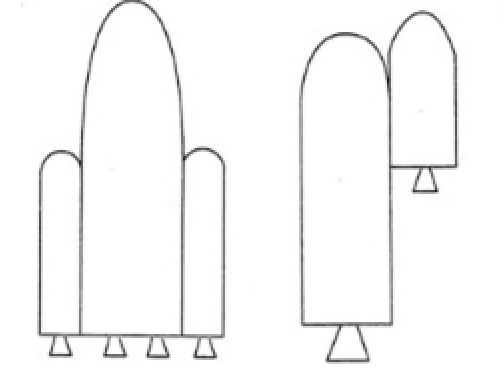
\includegraphics[scale=0.3]{image 15.png}
    \caption{Parallel staged rockets}
    \label{fig:parallel stage}
\end{figure}


\section{Interplanetary Trajectories}

\subsection{The Sphere of Activity}

When an object is "close enough" to the earth, it can be considered to orbit the earth.
When it is "far enough" away from the earth, it must be considered to orbit the sun.
Since in the patched conic method suggested by Hohmann, we shift point of view when an object is under that planet's control, it is necessary to investigate how large a volume of space is controlled by a particular planet. 
This is not an exact concept.

There is no actual boundary between gravitational fields of the earth and the sun, both affect the object. We can, however, formulate approximate definitions.

Consider the figure \ref{fig: activity sphere }

\begin{figure}[h]
    \centering
    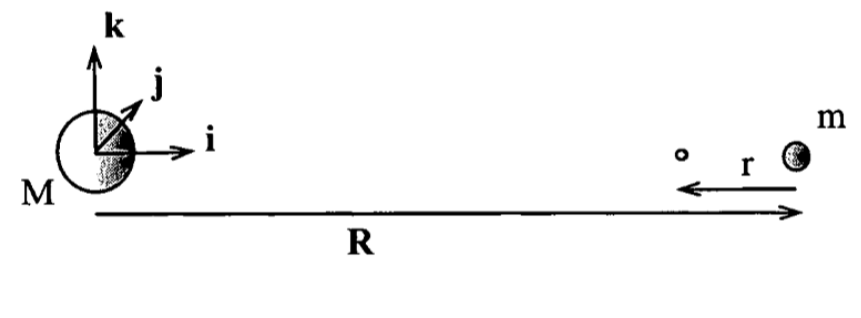
\includegraphics[scale=0.3]{image 16.png}
    \caption{Activity sphere calculation}
    \label{fig: activity sphere }
\end{figure}

The gravitational acceleration produced on the test mass by the sun and the planet is given by

\begin{equation}
    \boldsymbol{a}_g = - \frac{G M \boldsymbol{i}}{(R-r)^2} + \frac{G m \boldsymbol{i}}{r^2}
\end{equation}

We need to include the fact that both the planet and the test mass are themselves in orbit around the sun. 
By Kepler's third law, the angular velocity of the planet in circular orbit around the sun is

\begin{equation}
    \boldsymbol{\omega} =  \left( \frac{G M}{R^3} \right)^{1/2} \boldsymbol{k}
\end{equation}

Thus the centrifugal acceleration felt by the test mass is 

\begin{equation}
    \begin{split}
        \boldsymbol{a} & = \boldsymbol{\omega} \times (\boldsymbol{\omega} \times (R - r) \boldsymbol{i}) \\
        & = -\frac{G M}{R^3} (R - r) \boldsymbol{i}\\
    \end{split}
\end{equation}

We equate $a_g$ and $a$.

\begin{equation}
\begin{split}
    - \frac{G M }{(R-r)^2} + \frac{G m}{r^2} & = -\frac{G M}{R^3} (R - r) \\
     (R - r)^{-2} & \approx R^{-2} + 2 R^{-3} r \\
\end{split}   
\end{equation}

We now make the approximation  that $r$ is much smaller than $R$, and obtain the ratio $r/R$.

\begin{equation}
\begin{split}
    - 2 \frac{GM}{R^3}r + \frac{G m}{r^2} & = \frac{GM}{R^3}r\\
     \frac{r}{R} & \approx \left( \frac{m}{3M}\right)^{1/3}\\
\end{split}
\end{equation}

Here $r$ is the sphere of activity.

Another way of defining $r$ is as follows.

\begin{equation}
     \frac{r}{R} \approx \left( \frac{m}{3M}\right)^{2/5}
\end{equation}

The above equation is derived by a much more complex argument by Lagrange. 
The derivation has been skipped as it is extremely involving.

Both the definitions of the activity sphere are equally poor approximations.
However, it is still a decent approximation for our Solar system \emph{because the distances involved are very very large}.

It is used in the method of patched conics, where we assume that a spacecraft is influenced only by the gravitational field of the planet when it is within the activity sphere, and is influenced only by the gravity of the sun when it is outside any planet's activity sphere.

\subsection{Launch Windows and Mission Duration}

The Hohmann transfer is the best (minimum total $\Delta v$) route to follow for interplanetary transfers. 
However, it is certainly not the fastest way to reach the planets.
The Hohmann transfer is actually a local \emph{maximum} in the transfer time.

In general, while performing inter-planetary Hohmann transfers, it is desirable to arrive at the orbit of the second planet when that planet also arrives at that point.

\begin{figure}[h]
    \centering
    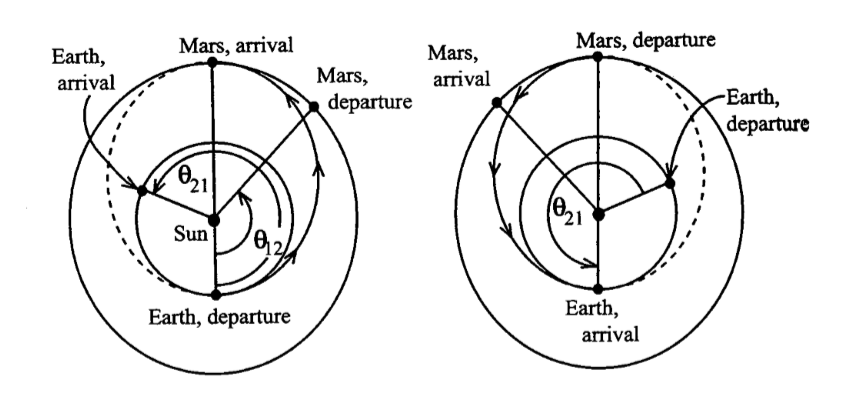
\includegraphics[scale=0.4]{image 17.png}
    \caption{Phase calculations}
    \label{fig:interplan}
\end{figure}

Consider the figure \ref{fig:interplan}.

Since the departure and arrival points are separated by $180\degree$, and since we know the transfer time $T_{12}$, the angle between the earth at launch and the planet \emph{at launch} can also be calculated.

If the planet moves along its orbit with mean motion $n_2$ then the phase angle at launch $\theta_{12}$ is given by the following.
\begin{equation}
 \theta_{12} = \pi - n_2 T_{12}
\end{equation}

(We define $\theta_{12}$ as the convenient reference object around is the planet).

The time when the earth is \emph{nearly} in this angular relationship to another planet is called the \emph{launch window} for that planet. 

Because of possible difficulties with artificial hardware and the weather, the booster must have some extra $\Delta v$ margin so that a less-than-optimal trajectory can be flown.
This excess booster capability would then determine the duration of the launch window.

The occurrence of a launch window to another planet can be found by calculating $\theta_{12}$ for the target object, then searching for dates when the earth and the planet will be in correct angular relationship. 

We define a term \emph{synodic period} which is given as follows.

\begin{equation}
    T_{syn} = \frac{2\pi}{|n_1 - n_2|}
\end{equation}

This gives the time taken by the earth to "lap" the target planet, or in case of the faster inner planets, the time taken to "lap" the earth.
It helps us find the launch windows (which occur at regular intervals).

In case of a manned mission to another planet we must provide for the return of the crew. 
we must do another Hohmann transfer for the return journey. 
The crew must wait at the target planet for the correct phase relation to occur, before the return journey.

Notice in the figure \ref{fig:interplan} the return transfer has just been rotated to align the positions earth at arrival and departure.

$\theta_{21}$ and $T_{wait}$ are as given below.
\begin{equation}
    \theta_{21} = n_1 T_{12}
\end{equation}

\begin{equation}
    T_{wait} = \frac{4\pi - 2\theta_{21}}{|n_2 - n_1|}
\end{equation}

\subsection{Departure and Arrival}

In the patched conic method, the crossing of an activity sphere boundary requires a change of reference frames.
At the point of crossing, the spacecraft ceases to be an earth orbiting object, and is now in orbit about the sun.

(Throughout this chapter, capitalized vectors are with respect to the sun, while lowercase vectors are with respect to a planet).

\begin{equation}\label{patch}
\begin{split}
    \boldsymbol{R} & = \boldsymbol{R}_0 + \boldsymbol{r}\\
    \boldsymbol{V} & = \boldsymbol{V}_0 + \boldsymbol{v}\\
\end{split}
\end{equation}

Here the subscript $0$ represents entity of the earth with respect to the sun.

The equations \ref{patch} are called \emph{patch conditions}.

While doing further calculations we make two assumptions. 
First, the activity sphere of the earth is much smaller than the size of the solar system.
Second, the activity sphere is much larger than the size of the earth and the spacecraft at the point on the activity sphere can be considered as escaped.

We generally use parking orbits, as they simplify maneuvers and calculations.
We get the advantage that there will be decently long interval each day during which an acceptable parking orbit can be achieved.
Also, the small errors that we commit, can be canceled by very small changes in the injection conditions in the parking orbit.

Arrival at the target planet is just the reverse of departure from the earth.
The main aim for arrival is to obtain the velocity of the space craft such that it is parallel to the planet's, after which necessary maneuvers are made.

\subsection{Planetary Flyby}

Until now, we have assumed that interplanetary trajectories would be minimum energy transfers. 
While the Hohmann transfer is the lowest energy option, it also takes the longest flight time.

In particular trip times are prohibitively long for the outer planets.
We can cut these times while also decreasing the total $\Delta v$ required.
A close flyby of one planets can radically alter the trajectory of the spacecraft after the flyby. 
The spacecraft can either gain or lose energy with respect to the sun, so that the new solar orbit can either reach much further out into the outer solar system, or drop considerably further inwards towards the inner planets.
In particular, a flyby of the most massive planet, Jupiter, can provide access to the entire solar system.

\begin{figure}[h]
    \centering
    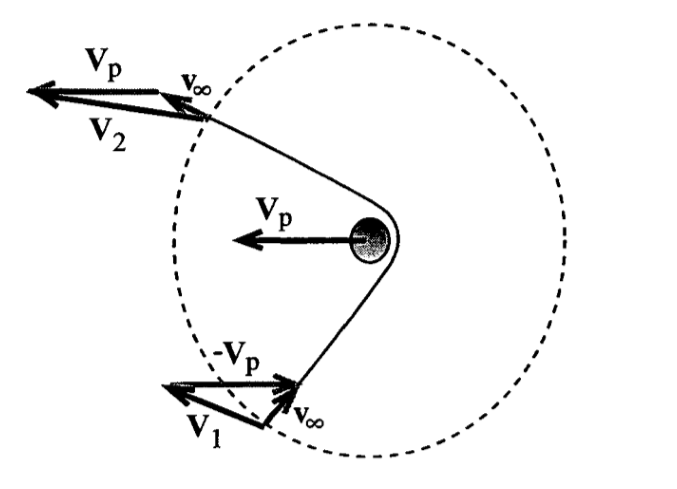
\includegraphics[scale=0.3]{image 18.png}
    \caption{Activity sphere crossing for flyby}
    \label{fig:flyby}
\end{figure}

Consider the figure \ref{fig:flyby}.
When the spacecraft crosses the activity sphere boundary, we must change our point of view and calculate the orbit of the spacecraft with respect to the planet.

Thus, 

\begin{equation}
\begin{split}
    \boldsymbol{r}_1 & = \boldsymbol{R}_1 - \boldsymbol{R}_p\\
    \boldsymbol{v}_1 & = \boldsymbol{V}_1 - \boldsymbol{V}_p\\
\end{split}
\end{equation}

Here $\boldsymbol{R}_1$ and $\boldsymbol{R}_p$ are the position vectors of the spacecraft and planet respectively to the sun, at the crossing time. 
$\boldsymbol{r}$ is the position vector of spacecraft with respect to planet. 
Likewise, for the velocity vector equation.

The flyby trajectory will always be a hyperbola with respect to the planet since the spacecraft approaches the planet from "infinitely" far away. 
If it does not hit the planet, it will recede from the planet, and again cross the activity sphere, passing back under the control of the sun.

At the outward crossing the position and velocity vectors of the spacecraft with respect to the sun are obtained as follows.

\begin{equation}
\begin{split}
    \boldsymbol{r}_2 & = \boldsymbol{R}_2 - \boldsymbol{R}_p\\
    \boldsymbol{v}_2 & = \boldsymbol{V}_2 - \boldsymbol{V}_p\\
\end{split}
\end{equation}

Note that $|\boldsymbol{v}_1|=|\boldsymbol{v}_2|=v_{escape}$.
The direction of both the velocity vectors may be greatly different.
In fact, for the case sketched in the figure, the new heliocentric speed is substantially larger than the speed at which the spacecraft originally approached the planet. 
This is characteristic of a \emph{trailing side} flyby of a planet.
We also call it a "gravitational slingshot".
A \emph{leading side} flyby, on the other hand can be considerably reduce the heliocentric speed of the probe.





\section{Reentry Dynamics}

The problem of surviving reentry does not arise in every space mission. 
Most earth satellites are given a one way ride out of the earth's atmosphere.
The spacecraft itself is not designed to survive reentry forces and heat loading.

However there are three cases where surviving reentry is of paramount importance. 
\begin{enumerate}
    \item Ballistic missile.
    \item Planetary entry probe.
    \item Manned spacecraft.
\end{enumerate}

The fundamental problem with reentry is the amount of kinetic energy per unit mass possessed by the spacecraft.
This energy must be dissipated effectively during reentry.

The spacecraft cannot be slowed to a stop with a rocket, since this would require a booster the size of the original launch vehicle. 
Instead we use atmospheric drag to slow the vehicle.

The rate at which drag dissipates energy is given by $D\cdot v$, which is proportional to $\rho v^3$. \medskip

There are two approaches for enduring the high temperatures generated by friction during atmospheric entry.
\begin{enumerate}
    \item We use the vehicle aerodynamics and the technology of the heat shield.
    \item Involves design of the reentry trajectory.
    By appropriate use of the dynamics the reentry can be stretched over a long time for disposing of waste heat.
\end{enumerate}

\subsection{Steep Ballistic Reentry}

\begin{figure}[h]
    \centering
    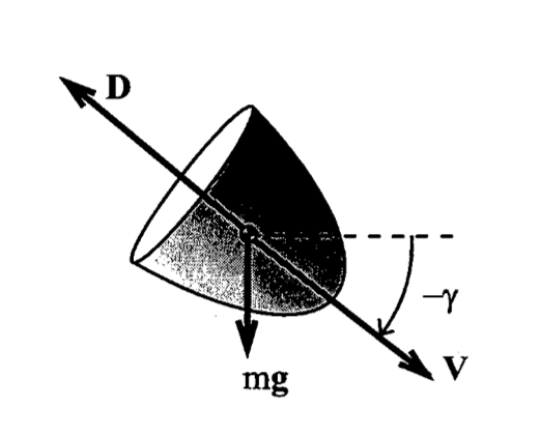
\includegraphics[scale=0.2]{image 19.png}
    \caption{Forces on a ballistic reentry vehicle}
    \label{fig:steep reentry}
\end{figure}

In this section we will consider the reentry of a ballistic vehicle without lift, for the case of steep entry angles.
Consider the figure \ref{fig:steep reentry}, it shows forces of gravity and drag.
We will call $X$ as downrange distance and $H$ as altitude. 

Let us conclude the equations of motion, in the downrange and vertical directions, as follows.

\begin{equation}
\begin{split}
    \frac{dX}{dt} & = V \cos{\gamma}\\
    \frac{dH}{dt} & = V \sin{\gamma}\\
\end{split}
\end{equation}

Considering in-track and cross-track accelerations we get the following equations.

\begin{equation}
\begin{split}
    m \frac{dV}{dt} & = -D -mg \sin{\gamma} \\
    m V \frac{d\gamma}{dt} & = -mg \cos{\gamma}\\
\end{split}
\end{equation}

If we switch to altitude $H$ being the independant variable, it will enable us to solve for the shape of the trajectory as a function of altitude.

\begin{equation}\label{steep1}
    \frac{dX}{dH} = \cot{\gamma} 
\end{equation}
\begin{equation}\label{steep2}
    m V \frac{dV}{dH} = - \frac{D}{\sin{\gamma}} - mg
\end{equation}
\begin{equation}\label{steep3}
    \frac{d\gamma}{dH}  = -\frac{g \cot{\gamma}}{V^2} 
\end{equation}

For the case of steep entry angles, the cotangent is small.
Also, velocity is likely to be large during most of the trajectory.

We will assume that $\gamma$ changes very little, as given in the equation \ref{steep3}. 
Equation \ref{steep1} also suggests that the trajectory is a straight line.

We will be concentrating on the deceleration.
$D$ here is found considering an exponential atmosphere and a hypersonic flight.

\begin{equation}
    D = \frac{1}{2} C_D A V^2\rho_0 e^{-H/H_0}
\end{equation}

Here $\rho_0$ is the atmospheric base density, $H_0$ is the scale height, and $A$ is the frontal area of the vehicle. Thus the equation \ref{steep2} becomes as follows.

\begin{equation}
m V \frac{dV}{dH} =  \frac{K_D}{H_0}\rho_0 e^{-H/H_0} - mg
\end{equation}

we have put $K_D$ as,

\begin{equation}
    K_D  = -\frac{C_D A H_0}{m \sin{\gamma_i}}
\end{equation}

The entry flight path angle $\gamma_i$ is assumed constant throughout the reentry trajectory, so $K_D$ is constant.




Using the assumptions and solving equation \ref{steep2} we get the following equation.

\begin{equation}
T_h = B_0 e^{-K_D \rho}
\end{equation}

Here $T_h$ is the kinetic energy for a particular $\rho$.
(The derivation has been skipped for brevity).

Here $B_0$ and $K_D$ are respectively given by 
\begin{equation}
    B_0  = m g H_0 Ei(K_D \rho)
\end{equation}

where the exponential integral function is defined as

\begin{equation}
Ei(x) = \int_{-\infty}^x \frac{e^x}{x}dx
\end{equation}

We will now evaluate the deceleration experienced by the reentry body.
This is a quantity of great interest to those who design the structure and contents of such a vehicle.

Since the vehicle does not experience acceleration due to gravity during free fall we can ignore the gravity terms in equation \ref{steep2}.

\begin{equation}
    a = -\frac{K_D \sin{\gamma_i} B_0}{m H_0} \rho e^{-K_D \rho}
\end{equation}

If we solve $da/d\rho = 0$ we get the maximum deceleration, and it occurs when $\rho = 1/K_D$.
\begin{equation}
    a_{max} = \frac{V_0^2 \sin{\gamma_i}}{2H_0 e}
\end{equation}

Note that this does not depend on $K_D$. \medskip

The case of low drag reentry bodies is important for the case of ballistic missile.
Low drag configurations are used since this minimizes the effects of trajectory curvature, and thus reduces any possible targeting error caused by local winds and atmospheric conditions.
By not slowing down this much, this configuration also minimizes atmospheric heating and deceleration structural loading.
Also, since the vehicle will approach the surface at high velocity, this approach is not useful for manned vehicles.

\begin{figure}
    \centering
    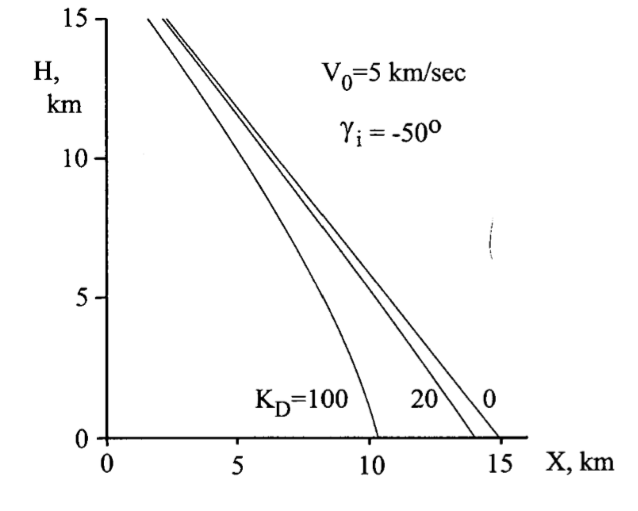
\includegraphics[scale=0.4]{image 20.png}
    \caption{Low drag ballistic trajectories}
    \label{fig:low drag}
\end{figure}

\medskip

A high drag vehicle will approach a quasi-equilibrium state during the last phase of the entry. 
In this state of near equilibrium, air drag will almost balance gravity.

Returning to equation \ref{steep2} and setting $\sin{\gamma_i} = -1$ for  vertical falling flight.

This implies,

\begin{equation}
    mV \frac{dV}{dH} = \frac{1}{2} C_D A V^2 \rho_0 e^{-H/H_0} -  mg \approx 0
\end{equation}

Solving this expression for the velocity, we find

\begin{equation}
    V_{lim} \approx \left(\frac{2mg}{C_D A \rho_0} \right)^{1/2} e^{H/2H_0}
\end{equation}

Just as in \emph{parachuting}, this is the terminal velocity of the reentry vehicle.
Note, however that the limiting velocity is an exponential function of the altitude above the ground.

\subsection{Shallow Planetary Probe Reentry}

At the opposite end of the reentry vehicle spectrum are planetary reentry probes and capsules designed to return from orbit.
Planetary have high values of $K_D$, and usually begin atmospheric entry at a shallow angle. 

Many such entry vehicles make observations on the chemistry and structure of the atmosphere during their descent.
This is difficult to do through the ionized sheath produced by hyper-sonic flight.

The entry probe must be decelerated rapidly, so that the atmospheric instruments can observe as much of the atmosphere as possible. 
The trajectory curves over sharply as the vehicle decelerates, and eventually the vehicle falls freely in the vertical direction.

The following two figures \ref{fig:mars1} and \ref{fig:mars2} demonstrate the landing of a rover on the Mars terrain.

\begin{figure}[h]
    \centering
    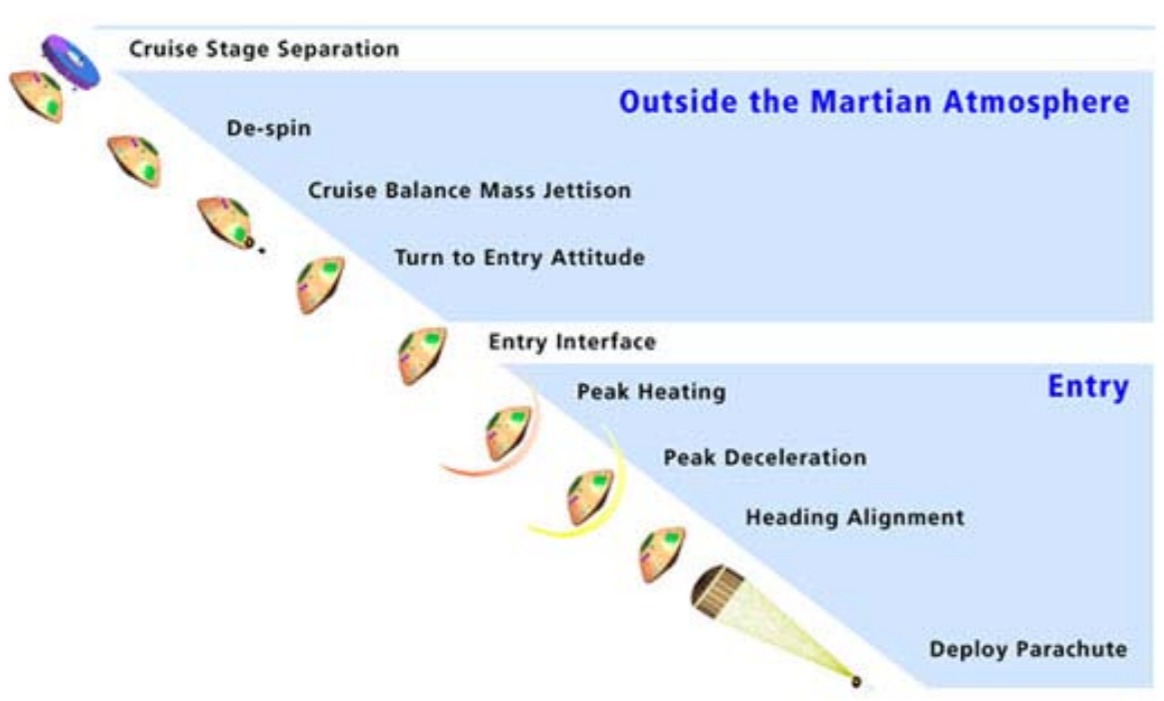
\includegraphics[scale=0.4]{full image 21.png}
    \caption{}
    \label{fig:mars1}
\end{figure}

\begin{figure}[h]
    \centering
    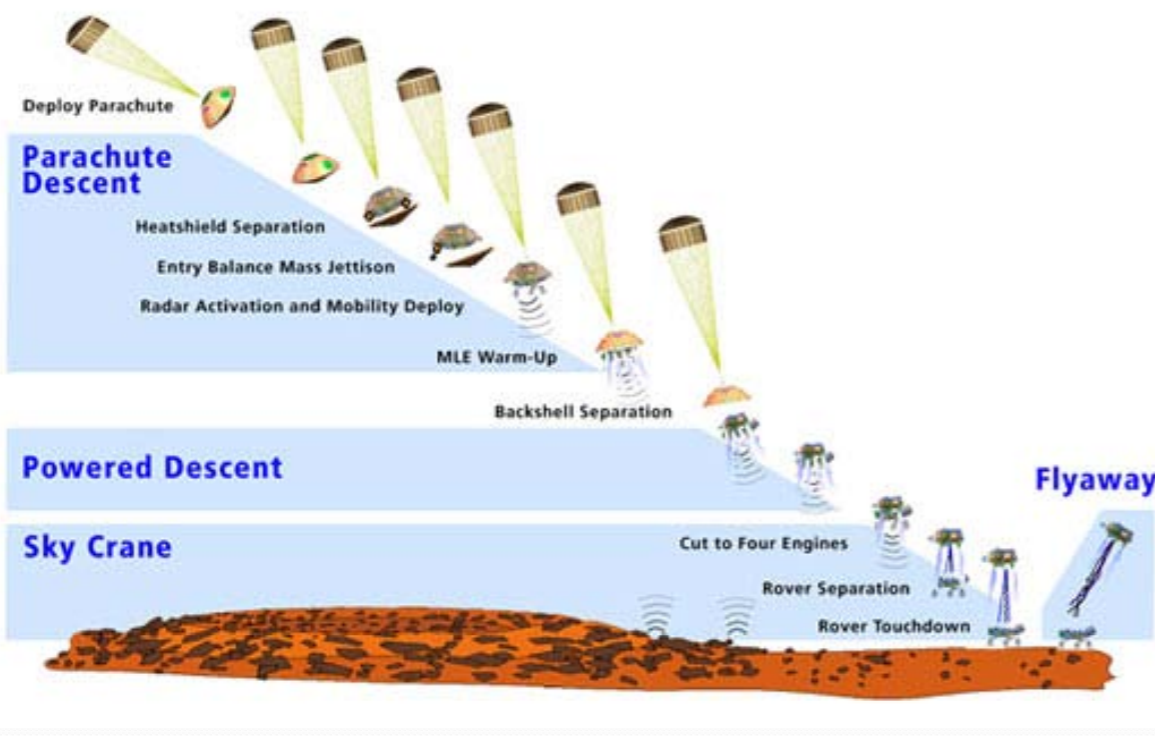
\includegraphics[scale=0.4]{full image 22.png}
    \caption{}
    \label{fig:mars2}
\end{figure}

\begin{thebibliography}{}
\bibitem{book}
\emph{(Mcgraw Hill Series in Aeronautical and Aerospace Engineering) William E. Wiesel} - Spaceflight Dynamics
\bibitem{lecture}
Lectures and notes by Professor Ashok Joshi on Spaceflight Mechanics
\bibitem{cdeep}
Lectures and notes by Professor H. Hablani on Spaceflight Mechanics
\end{thebibliography}


\end{document}

 